\documentclass[12pt,fleqn]{beamer}


\xdefinecolor{lavendar}{rgb}{0.8,0.6,1}
\xdefinecolor{olive}{cmyk}{0.64,0,0.95,0.4}
%\xdefinecolor{olive}{cmyk}{1,0,0,0}
\xdefinecolor{mag}{cmyk}{0.1,1,0,0.2}
\xdefinecolor{lblue}{rgb}{0,0,1.5}
\xdefinecolor{lred}{rgb}{1,0,0}
\xdefinecolor{mine}{cmyk}{1,0,0.2,0}
\xdefinecolor{bluel}{cmyk}{0.1,0,0.9,0.4}

\usepackage{amsmath,amssymb,dsfont,mathrsfs}
\usepackage{tikz,pgflibraryplotmarks}
\usepackage{multimedia}
\usepackage{wasysym}
\usepackage{rotating}
\usepackage{algorithm,algorithmic}
\usepackage{graphicx} % more modern
\usepackage{subfigure}
\usepackage{booktabs}

\usepackage{pgfplots}
\usepackage{verbatim}

\usepackage{setspace}
\newlength\iwidth
\newlength\iheight

\newcommand\makebeamertitle{\frame{\maketitle}}%
\graphicspath{{./images/}}
\setbeamertemplate{navigation symbols}{}
\addtobeamertemplate{navigation symbols}{}{%
    \usebeamerfont{footline}%
    \usebeamercolor[fg]{footline}%
	\insertshorttitle
    \;--
    \insertframenumber
}

\newcommand{\sectionstart}{
	\only<beamer>{
 	\begin{frame}% (fold)
 		\begin{centering}\Huge \insertsection \par\end{centering}
 	\end{frame}% frame the_application (end)
	}
 }


% make bibliography entries smaller
\usepackage{natbib}
\setbeamertemplate{bibliography item}{[\theenumiv]}
\renewcommand\bibfont{\scriptsize}
\setbeamertemplate{frametitle continuation}[from second]
\newcommand{\tcr}{\textcolor{red}}
\newcommand{\tcrd}{\textcolor{red}}
\newcommand{\tcb}{\textcolor{bluel}}
\newcommand{\tcm}{\textcolor{mag}}
\newcommand{\tcg}{\textcolor{olive}}

\newcommand{\R}{\mathbb{R}}
\newcommand{\C}{\mathbb{C}}

% bold lower-case for vectors
\newcommand{\bfa}{{\bf a}}
\newcommand{\bfb}{{\bf b}}
\newcommand{\bfc}{{\bf c}}
\newcommand{\bfs}{{\bf s}}
\newcommand{\bfm}{{\bf m}}
\newcommand{\bfd}{{\bf d}}
\newcommand{\bfe}{{\bf e}}
\newcommand{\bfu}{{\bf u}}
\newcommand{\bfy}{{\bf y}}
\newcommand{\bfx}{{\bf x}}
\newcommand{\bfh}{{\bf h}}
\newcommand{\bfw}{{\bf w}}
\newcommand{\bfv}{{\bf v}}
\newcommand{\bfr}{{\bf r}}
\newcommand{\bfz}{{\bf z}}
\newcommand{\bfp}{{\bf p}}


% bold upper-case for linear operators
\newcommand{\bfA}{{\bf A}}
\newcommand{\bfB}{{\bf B}}
\newcommand{\bfZ}{{\bf Z}}
\newcommand{\bfM}{{\bf M}}
\newcommand{\bfC}{{\bf C}}
\newcommand{\bfD}{{\bf D}}
\newcommand{\bfQ}{{\bf Q}}
\newcommand{\bfJ}{{\bf J}}
\newcommand{\bfG}{{\bf G}}
\newcommand{\bfI}{{\bf I}}
\newcommand{\bfP}{{\bf P}}
\newcommand{\bfK}{{\bf K}}
\newcommand{\bfY}{{\bf Y}}
\newcommand{\bfW}{{\bf W}}
\newcommand{\bfR}{{\bf R}}
\newcommand{\bfL}{{\bf L}}
\newcommand{\bfF}{{\bf F}}
\newcommand{\bfT}{{\bf T}}
\newcommand{\bfS}{{\bf S}}
\newcommand{\bfX}{{\bf X}}
\newcommand{\bfU}{{\bf U}}
\newcommand{\bfV}{{\bf V}}
\newcommand{\bfH}{{\bf H}}


\newcommand{\calF}{\mathcal{F}}



\newcommand{\hf}{{\frac 12}}
\newcommand{\bftheta}{{\boldsymbol \theta}}
\newcommand{\bfxi}{{\boldsymbol \xi}}

\newcommand{\bfLambda}{{\boldsymbol \Lambda}}
\newcommand{\bfSigma}{{\boldsymbol \Sigma}}
\newcommand{\bfepsilon}{{\boldsymbol \epsilon}}

\newcommand{\E}{\vec E}
\newcommand{\B}{\vec B}

\newcommand{\vu}{  {\vec {\bf u}}}

\newcommand{\grad}{  {\vec {\bf \nabla}}}

\newcommand{\lfrownie}{\textcolor{red}{\large{\frownie}}}
\newcommand{\lsmiley}{\textcolor{green}{\large{\smiley}}}

\newcommand{\curl}{\ensuremath{\nabla\times\,}}
\renewcommand{\div}{\nabla\cdot\,}
\newcommand{\divh}{\nabla_h\cdot\,}
\renewcommand{\grad}{\ensuremath{\nabla}}

\DeclareMathOperator*{\argmin}{arg\,min}


\title{Training Single Layer Neural Networks}
\subtitle{Numerical Methods for Deep Learning}
\date{}
\begin{document}

\makebeamertitle


\begin{frame}[fragile]\frametitle{Overview}

Given data $\bfY \in \R^{n_f\times n}$ and class probabilities $\bfC\in\R^{n_c\times n}$ we aim to find the transformation parameters $\bftheta\in\R^p$ and classification weights (including potentially biases) $\bfW \in \R^{n_c \times m}$ by solving
$$
\min_{\bftheta,\bfW} E(\bfW \sigma(\bfK(\bftheta)\bfY), \bfC) + \lambda R(\bftheta,\bfW)
$$

Today: Derive practical pipeline consisting of 
\begin{itemize}
	\item variable projection
	\item Stochastic Average Approximation (SAA)
	\item regularization
\end{itemize}


\end{frame}

\begin{frame}\frametitle{Variable Projection - 1}
	Idea: Treat learning problem as coupled optimization problem with blocks $\bftheta$ and $\bfW$. 
	
	Simple illustration for coupled least-squares problem~\cite{GoPe1973,GoPe03,OLearyRust2013}
	$$
		\min_{\bftheta,\bfw} \phi(\bftheta,\bfw) = \hf \| \bfA(\bftheta) \bfw - \bfc\|^2 + \frac{\lambda}{2}\| \bfL \bfw\|^2 + \frac{\beta}{2} \| \bfM \bftheta\|^2
	$$
	Note that for given $\bftheta$ the problem becomes a standard least-squares problem. Define: 
	$$
		\bfw(\bftheta) = \left( \bfA(\bftheta)^\top \bfA(\bftheta) + \lambda \bfL^\top \bfL \right)^{-1}{\bfA(\bftheta)^\top \bfc}
	$$
	This gives optimization problem in $\bftheta$ only (aka \emph{reduced/projected  problem})
	$$
		\min_{\bftheta} \tilde{\phi}(\bftheta) = \hf \| \bfA(\bftheta) \bfw(\bftheta) - \bfc\|^2 + \frac{\lambda}{2}\| \bfL \bfw(\bftheta)\|^2 + \frac{\beta}{2} \| \bfM \bftheta\|^2
	$$
	
\end{frame}
\begin{frame}\frametitle{Variable Projection - 2}
	$$
		\min_{\bftheta} \tilde{\phi}(\bftheta) = \hf \| \bfA(\bftheta) \bfw(\bftheta) - \bfc\|^2 + \frac{\lambda}{2}\| \bfL \bfw(\bftheta)\|^2 + \frac{\beta}{2} \| \bfM \bftheta\|^2
	$$
	Optimality condition:
	$$ 
		\nabla \tilde{\phi}(\bftheta) = \nabla_\bftheta \phi(\bftheta,\bfw) + \nabla_\bftheta \bfw(\bftheta) \nabla_{\bfw} \phi(\bftheta,\bfw) \stackrel{!}{=} 0.
	$$
	Less complicated than it seems since
	$$
		\nabla_{\bfw} \phi(\bftheta,\bfw(\bftheta)) = \bfA(\bftheta)^\top( \bfA(\bftheta) \bfw(\bftheta) - \bfc) + \lambda \bfL^\top \bfL \bfw(\bftheta) = 0
	$$
	
	Conclusion:
	\begin{itemize}
		\item ignore second term in gradient computation
		\item apply steepest descent or Gauss-Newton  to minimize $\tilde{\phi}$
		\item need to solve least-squares problem in each evaluation of objective
		\item gradient is only correct if LS problem is solved exactly
	\end{itemize}
	
\end{frame}

\begin{frame}
	\frametitle{Variable Projection for Single Layer}
	
$$
\min_{\bftheta,\bfW} E(\bfW \sigma(\bfK(\bftheta)\bfY ), \bfC) + \lambda R(\bftheta,\bfW)
$$
Assume that the regularizer is separable, i.e.,
$$
 R(\bftheta,\bfW) =   R_1(\bftheta) +  R_2(\bfW)
$$
and that $R_2$ is convex and smooth. Hence, the projection requires solving the regularized classification problem
$$
\bfW(\bftheta) = \argmin_{\bfW} E(\bfW\sigma(\bfK(\bftheta)\bfY), \bfC) + \lambda R_2(\bfW)
$$
practical considerations:
\begin{itemize}
	\item solve for $\bfW(\bftheta)$ using Newton (need accuracy)
	\item need good solver to approximate gradient w.r.t. $\bftheta$  well
	\item use Gauss-Newton or steepest descent to solve for $\bftheta$ 
\end{itemize}
\end{frame}

\begin{frame}[fragile]\frametitle{Stochastic Optimization}
	Assume that each $\bfy_i$, $\bfc_i$ pair is drawn from some (unknown probability distribution). 
	
	Then, we can interpret the learning problem as minimizing the expected value of the cross entropy, e.g., in linear regression
	$$
		E(\bfW) = {\mathbb{E}} \left(\hf \|\bfy^\top \bfW - \bfc\|^2\right)
	$$
	
	This is a stochastic optimization problem~\cite{bottou2016optimization}. \pause One idea: \textbf{Stochastic Approximation: } Design iteration $\bfW_k \to \bfW^*$ so that expected value decreases.
		
		Example: Stochastic Gradient Descent, ADAM, \ldots
		
		Pro: sample can be small (\emph{mini batch})
		
		Con: how to monitor objective, linesearch, descent, \ldots
\end{frame}
\begin{frame}
	\frametitle{Stochastic Average Approximation}
	
	Alternative way to solve stochastic optimization problem
	$$
	E(\bfW) = {\mathbb{E}} \left(\hf \|\bfy^\top \bfW - \bfc\|^2\right)
	$$
	
	 Pick relatively large sample $S \subset \{ 1,\ldots,n\}$ and use deterministic optimization method to solve
			$$
				\min_\bfW  \frac{1}{2|S|} \sum_{s\in S} \| \bfy_s \bfW - \bfc_s^\top \|^2.
			$$
		
			Pro: use your favorite solver, linesearch, stopping\ldots
			
			Con: large batches needed
			
			\begin{center}
				Note: Sample stays fixed during iteration.
			\end{center}
\end{frame}
\begin{frame}
	\frametitle{A Practical Approach}
	
	Let's combine VarPro and SAA to come up with a simple yet powerful training algorithm.
	
	\bigskip
	\pause
	
	Pick $(\bftheta_0)$ randomly and then do one or more steps of:
	\begin{enumerate}
		\item randomly select samples $S$ (large enough)
		\item do a few steps of variable projection to get $\bftheta_k$.
		\begin{itemize}
			\item inner solver: a few steps of Newton's method
		\end{itemize}
		\item check training error on current batch and validation error
	\end{enumerate}
	
	\bigskip
	\pause
	
	Possible problems:
	\begin{itemize}
		\item $|S|$ too small $\rightarrow$ training error small but no convergence
		\item $|S|$ too large $\rightarrow$ slow, overfitting (use regularization)
		\item Too few Newton steps in classification $\rightarrow$ inaccurate gradients, line search fails, \ldots
	\end{itemize}	
\end{frame}

\begin{frame}[fragile]\frametitle{Data Preprocessing}

Some practical tips
\begin{itemize}
\item Remove the mean of the data
\item Scale it to be ``reasonable'' scale
\item Data augmentation
\item Some other (domain specific) data transforms (optical flow for motion?)
\end{itemize}

\end{frame}

\begin{frame}[fragile]\frametitle{Regularization for Network Weights}

\begin{itemize}
\item
Note that there are many more degrees of freedom.
\item
Need to add regularization for $\bfK$
\item
$\bfK$ Generally, $\bfK$ is not ``physical'' - difficult to choose reasonable
regularization.
\end{itemize}

\bigskip

The obvious choice: Tikhonov
$$ R(\bfK) = \hf \|\bfK\|^2_F $$
(also called weight decay)


\end{frame}

\begin{frame}[fragile]\frametitle{Learning the weights - Regularization}

\begin{columns}
	\column{.7\textwidth}
More recent, demand that $\bfK$ is sparse
$$ R(\bfK) = \|{\rm vec}(\bfK)\|_1 = \sum_{ij} |\bfK_{ij}| $$

\bigskip

Implementation through soft-thresholding.


After each steepest descent iteration set
$$ \bfK = {\rm softThresh}(\bfK) $$
	
	\column{.3\textwidth}
	\begin{center}
	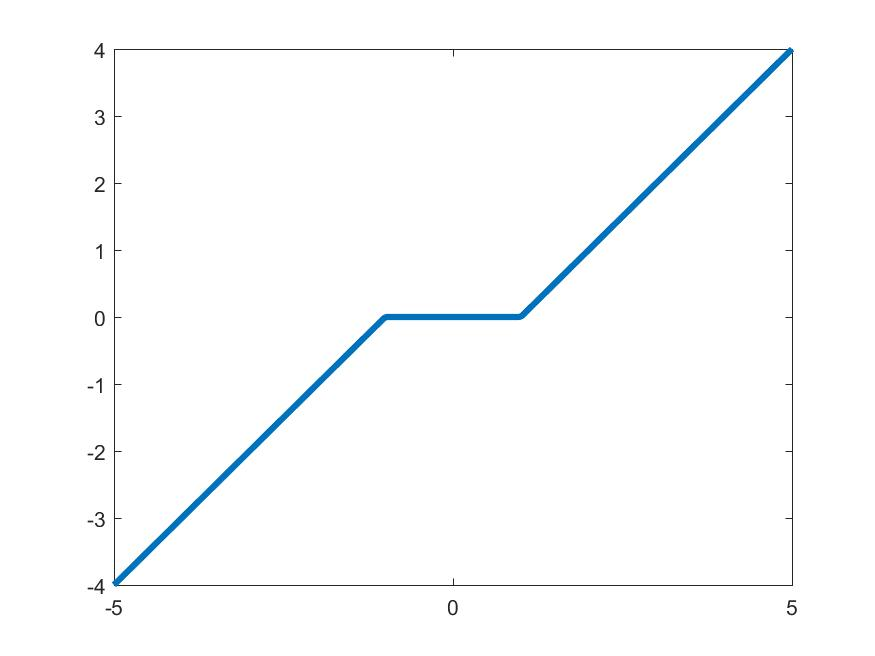
\includegraphics[width=4cm]{shoftThresh.jpg}
	\end{center}
	
\end{columns}

\vspace{10mm}
\begin{center}
Obtain sparse matrices $\bfK$ that retain only necessary entries
	
\end{center}

\end{frame}




\begin{frame}[fragile]\frametitle{Coding: Learning the weights }

{\bf Class problem}

\bigskip

Modify your steepest descent, nonlinear CG and SGD codes to work on single layer
network with soft thresholding.

Test on Circle, peaks, spiral, MNIST and CIFAR10

Compare and report

\end{frame}
\begin{frame}\frametitle{Experiment: Peaks}
	
	Compare the three approaches for training a single layer neural network
	
	\begin{itemize}
		\item \texttt{ESingleLayer\_PeaksSGD.m} - stochastic gradient descent 
		\item \texttt{ESingleLayer\_PeaksNewtonCG.m} - Newton CG with block-diagonal Hessian approximation
		\item \texttt{ESingleLayer\_PeaksVarPro.m} - Fully coupled solver. Eliminate $\bftheta$ and use steepest descent/Newton CG for reduced problem.
	\end{itemize}
	
\end{frame}



% \begin{frame}[fragile]
% 	\frametitle{Other Hints}
%
% 	To accelerate convolutions, you may want to use GPUs. Learn more at
% 	\begin{verbatim}
% 		https://www.mathworks.com/discovery/matlab-gpu.html
% 	\end{verbatim}
%
% 	Systems set up in the computer lab:
% 	\begin{itemize}
% 		\item \texttt{lab3f, lab3g, lab3h}
% 		\item make sure to use recent Matlab (hint on exercise sheet)
% 	\end{itemize}
%
% 	Also possible to use Cloud: Example setup
% 	\begin{itemize}
% 		\item instance with 2 cores, lots of RAM, $\geq 30$ GB disk, cheaper NVIDIA GPU $\approx$ 0.5\$ per hour and Ubuntu 16.04
% 		\item you need to install MATLAB and CUDA
% 	\end{itemize}
%
% \end{frame}

\begin{frame}[allowframebreaks]
	\frametitle{References}
\bibliographystyle{abbrv}
\bibliography{NumDNN}

\end{frame}

\end{document}




















